\documentclass{article}
% \documentclass[UTF8]{ctexart}
\usepackage{amsmath,amssymb,amsfonts}  % For math symbols and fonts
\usepackage{graphicx}                   % For including images
\usepackage{hyperref}                   % For hyperlinks
\usepackage{cite}                       % For citations
\usepackage[UTF8]{ctex}  % 注意,不是 \documentclass[UTF8]{ctexart}

\usepackage{algorithm}
\usepackage{algorithmic}

\usepackage{amsthm}
% Define new theorem-like environments
% Define environments
\theoremstyle{definition} % Non-italicized style
\newtheorem{definition}{Definition}[section]
\newtheorem{exercise}{Exercise}[section]

% Title and author info
\title{Makes drones in cirle Experiments Report}
\author{
Zhang Jinrui\thanks{alternative email:zhangjr1022@mails.jlu.edu.cn} \\ \texttt{jerryzhang40@gmail.com}
\\Su Zinan \\ \texttt{suzinan20050803@aliyun.com}
\\Xu Haoran\thanks{alternative email:Xuhr1023@mails.jlu.edu.cn} \\ \texttt{haoranxu288@gmail.com}
}

\date{20250720}  % Empty date; optional, you can also specify a date here

\begin{document}

\maketitle

\begin{abstract}
    In this article, I tried to do apply a
    simple policy to each drone to make
    them fly in cirle
\end{abstract}

\section{recite of the problem \& assumptions}
There are 10 drones and fly on the sky
obeys Newton's second law of motion.
which is
\[
    \vec{F} = m \vec{a}
\]
\[
    \vec{a} = \frac{d\vec{v}}{dt} = \frac{d^2 \vec{x}}{dt^2}
\]
And I mean the policy by, we need a function of force
depending on some communication between drones
to decide the \(\vec{F}\)
\[
    \vec{F}=f(the current information)
\]

And then we want the following dynamic system
\[\begin{bmatrix}
        \frac{d\vec{d}}{dt} \\
        \frac{d\vec{v}}{dt}
    \end{bmatrix}=
    \begin{bmatrix}
        \vec{v} \\
        \vec{a}=f/m
    \end{bmatrix}
\]
has some Self-organized emergent phenomena,
to automatically emergent a circle rounding pattern.

\section{a simple prompt}
To be more clear of the notations we use,
we have \(i\in\{1,2,...,10\}=N\)
And the drones are ignored of its flying
height, which the position vector can be a
2d vector note it as \(\vec{d_i}\)
And so the velocity and acceleration we denote as
\(\vec{v_i}=\frac{d\vec{d_i}}{dt}\)
and
\(\vec{a_i}=\frac{d\vec{v_i}}{dt}\)
I want to prompt a \(f\) so that it can form
a cirle.
\[
    \vec{f_i}=m_i(\sum_{\forall k\neq i,\|\vec{d_i}-\vec{d_k}\|\leq R}(\frac{\vec{d_i}-\vec{d_k}}{\|\vec{d_i}-\vec{d_k}\|^3})+(\frac{\vec{d_{t(i)}}-\vec{d_i}}{\|\vec{d_{t(i)}}-\vec{d_i}\|}-v_i))
\]
This model is easy to explain, the first term is
just a inverse square propell force, the second
term is make the velocity quickly approch a set direction
the \(t(i)\) is just a randomly choosed target drone
other than \(i\) that is \(t(i)\in N, t(i)\neq i\)

This formula can be rewrite without physical term as
follow.
\[
    \vec{a_i}=\sum_{\forall k\neq i,\|\vec{d_i}-\vec{d_k}\|\leq R}(\frac{\vec{d_i}-\vec{d_k}}{\|\vec{d_i}-\vec{d_k}\|^3})+(\frac{\vec{d_{t(i)}}-\vec{d_i}}{\|\vec{d_{t(i)}}-\vec{d_i}\|}-v_i)
\]
separately view this is combined by two independent force
\[
    (\vec{a_i})_{target}=(\frac{\vec{d_{t(i)}}-\vec{d_i}}{\|\vec{d_{t(i)}}-\vec{d_i}\|}-v_i)
\]
\[
    (\vec{a_i})_{propell}=\sum_{\forall k\neq i,\|\vec{d_i}-\vec{d_k}\|\leq R}(\frac{\vec{d_i}-\vec{d_k}}{\|\vec{d_i}-\vec{d_k}\|^3})
\]

\section{a simple prompt:simulation}
\subsection{Four drone case}
\subsubsection{derivation}
This case just choose \(N=\{1,2,3,4\}\)
and don't allow \(t(t(i))=i\)
which definitely form a three element loop and
a dangling drone.

We have a (4,2)-tensor \(\vec{d_i}\)
and two other (4,2)-tensor \(\vec{v_i}\)
and \(\vec{a_i}\)
The initial points are randomly choosed
in Uniformly \([0,1]\times[0,1]\)

choose a time increment \(dt\)
and the simulation update formula is simple to write

just as follow
\[\begin{bmatrix}
        \vec{{d_{n+1}}_i} \\
        \vec{{v_{n+1}}_i}
    \end{bmatrix}=
    \begin{bmatrix}
        \vec{{d_{n}}_i}+\vec{{v_n}_i}dt \\
        \vec{{v_{n}}_i}+(\sum_{\forall k\neq i,\|\vec{{d_n}_i}-\vec{{d_n}_k}\|\leq R}(\frac{\vec{{d_n}_i}-\vec{{d_n}_k}}{\|\vec{{d_n}_i}-\vec{{d_n}_k}\|^3})+(\frac{\vec{{d_n}_{t(i)}}-\vec{{d_n}_i}}{\|\vec{{d_n}_{t(i)}}-\vec{{d_n}_i}\|}-{v_n}_i))dt
    \end{bmatrix}
\]

simple Euler method.
\subsubsection{code \& result}
the computational code are \cite[FourDroneCase]{FourDroneCase} .
the results are shown by the following pictrues which
generated by the code.
The video are \cite[sample1-video]{sample1-video}
and \cite[sample2-video]{sample2-video}
and more other in the same folder on github.
\begin{figure}[ht!]
    \centering
    \begin{minipage}{0.45\textwidth}
        \centering
        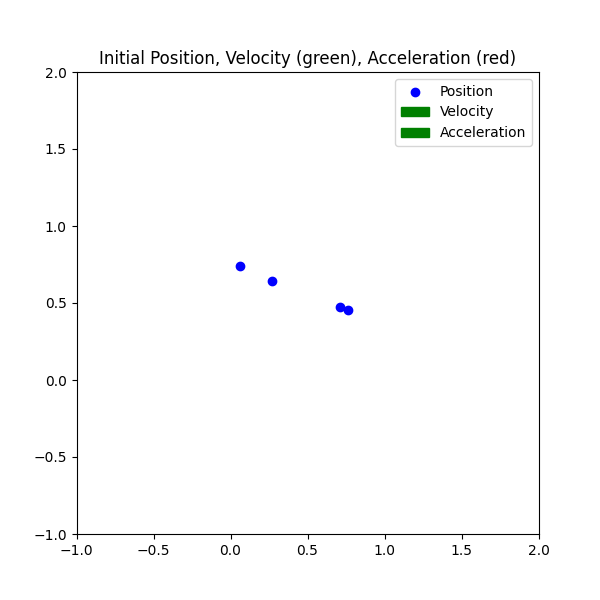
\includegraphics[width=0.9\textwidth]{fig/sample1/dd.png} % first figure itself
        \caption{sample1 randomly initial position}
        \label{fig:fig1}
    \end{minipage}\hfill
    \begin{minipage}{0.45\textwidth}
        \centering
        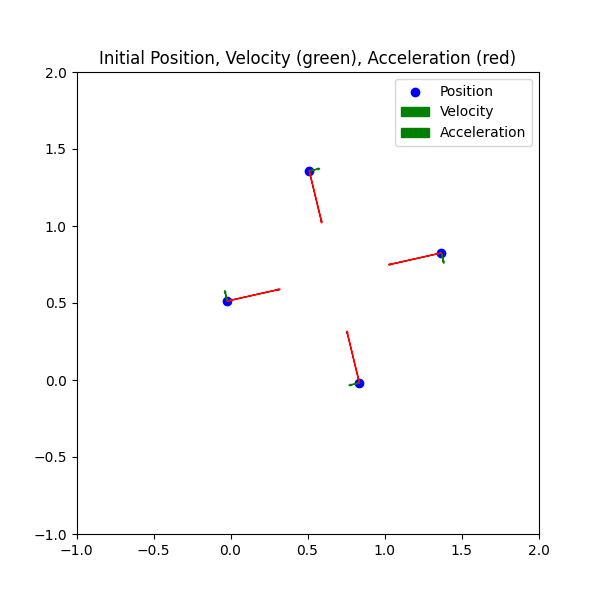
\includegraphics[width=0.9\textwidth]{fig/sample1/dd_18254.png} % second figure itself
        \caption{sample1 after a period of time}
    \end{minipage}
\end{figure}
\begin{figure}[ht!]
    \centering
    \begin{minipage}{0.45\textwidth}
        \centering
        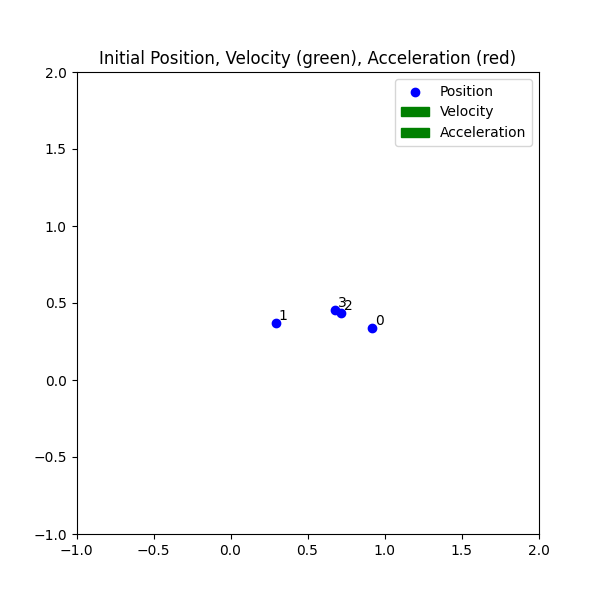
\includegraphics[width=0.9\textwidth]{fig/sample2/dd.png} % first figure itself
        \caption{sample1 randomly initial position}
        \label{fig:fig2}
    \end{minipage}\hfill
    \begin{minipage}{0.45\textwidth}
        \centering
        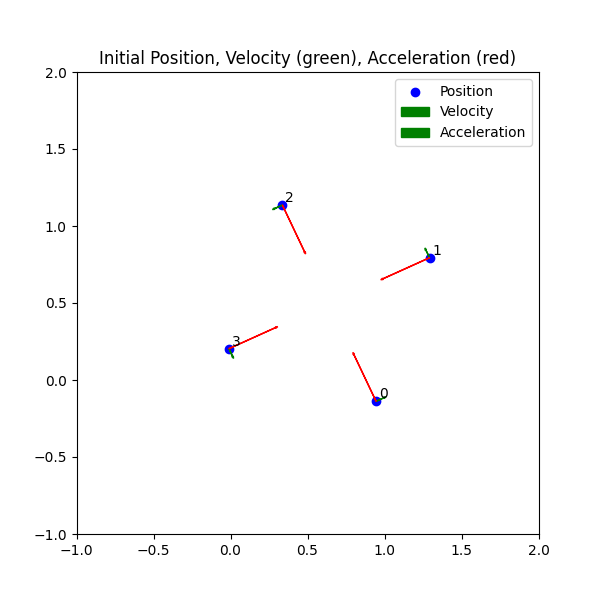
\includegraphics[width=0.9\textwidth]{fig/sample2/dd_18993.png} % second figure itself
        \caption{sample2 after a period of time}
    \end{minipage}
\end{figure}

\subsection{Ten drone case}
undergoing
\subsubsection{derivation}
undergoing

\section{some analysis why it will have a stability property}
\subsection{the terminate radius R}
undergoing
\subsection{the terminate center O}
undergoing
\subsection{graph theory part}
The \(t(i)\) forms a graph which have \(n\) points
and \(n\) oriented edges, this forms a tree with a extra
edges, and this case It will obviously form a Unicyclic Graph.

Which is a tree if we treat all the point on the
loop as the same point.

\section{Zinan Su's approach}
\subsection{notations \& equations}
safe collide radius is \(d_s\)
\[
    \sigma=2d_s
\]
\(NUM\) is the total number of the drones.
And then we want the following dynamic system
\[\begin{bmatrix}
        \frac{d\vec{p_i}}{dt} \\
        \frac{d\vec{v_i}}{dt}
    \end{bmatrix}=
    \begin{bmatrix}
        \vec{v_i} \\
        \vec{a_i}
    \end{bmatrix}
\]
circle origin is a function
\[
    c=\frac{1}{NUM}\sum_{k=1}^{NUM}p_k
\]
Four constants.
\[
    k_p=
\]
\[
    k_d=
\]
\[
    k_v=
\]
\[
    k_r=
\]
\[
    R^*=\frac{1}{NUM}\sum_{k=1}^{NUM}p_k(0)-c(0)
\]
\[
    v_d=\frac{1}{NUM}\sum_{k=1}^{NUM}\|v_k(0)\|
\]
and
\[
    r_i=p_i-c
\]
\[
    d_i=\|r_i\|
\]
\[
    \hat{r_i}=\frac{r_i}{d_i}
\]
\[
    \hat{\theta_i}=\mathbb{M}_\theta r_i
\]
\[
    \mathbb{M}_\theta=
    \begin{bmatrix}
        0  & 1 \\
        -1 & 0
    \end{bmatrix}
\]
\[
    {v_{i}}_{\parallel}=\hat{r_i}\cdot v_i
\]
\[
    {v_{i}}_{\perp}=\hat{\theta_i}\cdot v_i
\]
\[
    U(r)=k_re^{-\frac{r}{2\sigma^2}}
\]
\[
    U_{ij}=U(\|p_i-p_j\|)
\]
\[
    \vec{u_i}_1=[-k_p(d_i-R^*)-k_d{v_{i}}_{\parallel}]\hat{r_i}
\]
\[
    \vec{u_i}_2=[-k_v({v_{i}}_{\perp}-v_d)]\hat{\theta_i}
\]
\[
    \vec{u_i}_3=\sum_{\forall k\neq i}(-\nabla_{p_i}U_{ij})
\]
\[
    \vec{u_i}=\vec{u_i}_1+\vec{u_i}_2+\vec{u_i}_3
\]

\subsection{analysis}
考虑带阻力的动力方程
\begin{equation*}
    m\frac{\mathrm{d}^2\boldsymbol{p}_i}{\mathrm{d}t^2}+c\left\|\frac{\mathrm{d}\boldsymbol{p}_i}{\mathrm{d}t}\right\|\frac{\mathrm{d}\boldsymbol{p}_i}{\mathrm{d}t}=\boldsymbol{u}_i,
\end{equation*}
其中 $m$ 为质量, $c$ 为阻力系数, 即
\begin{align}
    \frac{\mathrm{d}\boldsymbol{X}}{\mathrm{d}t}=\boldsymbol{F}(\boldsymbol{X}),
\end{align}
其中
\begin{equation*}
    \boldsymbol{X}=\binom{\boldsymbol{p}}{\boldsymbol{v}}\in\mathbb{R}^{40},\ \boldsymbol{p}=\begin{pmatrix}
        \boldsymbol{p}_1 \\\vdots\\\boldsymbol{p}_{10}
    \end{pmatrix},\ \boldsymbol{v}=\begin{pmatrix}
        \boldsymbol{v}_1 \\\vdots\\\boldsymbol{v}_{10}
    \end{pmatrix},\ \boldsymbol{F}(\boldsymbol{X})=\binom{\boldsymbol{v}}{m^{-1}(\boldsymbol{u}-c\|\boldsymbol{v}\|\boldsymbol{v})}.
\end{equation*}
易知质心 $\boldsymbol{c}(\boldsymbol{X}),\|\boldsymbol{r}_i\|,\widehat{\boldsymbol{r}_i},\mathit{\Phi}$ 均为 Lipschitz 连续函数, 且初值条件满足
\begin{equation*}
    \min_{i\ne j}\|\boldsymbol{p}_i(0)-\boldsymbol{p}_j(0)\|>d_s>0.
\end{equation*}
由 Picard 定理可知方程 (1) 的解存在且唯一, 解为
\begin{equation*}
    \boldsymbol{X}(t)=\boldsymbol{X}(0)+\int_0^t\boldsymbol{F}(\boldsymbol{X}(s))\mathrm{d}s,
\end{equation*}
即
\begin{align*}
     & \boldsymbol{v}_i(t)=\boldsymbol{v}_i(0)+\int_0^t\left[m^{-1}\boldsymbol{u}_i(\boldsymbol{X}(s))-\frac{c}{m}\|\boldsymbol{v}_i(s)\|\boldsymbol{v}_i(s)\right]\mathrm{d}s, \\
     & \boldsymbol{p}_i(t)=\boldsymbol{p}_i(0)+\int_0^t\boldsymbol{v}_i(s)\mathrm{d}s.
\end{align*}
下面证明防撞性. 定义
\begin{align*}
     & \mathit{\Psi}(d)=k_r\exp\left\{-\frac{(d-d_s)^2}{2\sigma^2}\right\},                                                                      \\
     & \mathit{\Phi}(d)=-\frac{\mathrm{d}\mathit{\Psi}}{\mathrm{d}d}=\frac{k_r}{\sigma^2}\exp\left\{-\frac{(d-d_s)^2}{2\sigma^2}\right\}(d-d_s), \\
     & E_{ij}(t)=\frac{1}{2}\left(\frac{\mathrm{d}d_{ij}}{\mathrm{d}t}\right)^2+\psi(d_{ij}(t)),
\end{align*}
其中 $d_{ij}(t)=\|\boldsymbol{p}_i(t)-\boldsymbol{p}_j(t)\|.$ 则系统能量为
\begin{equation*}
    \mathcal{E}(t)=\sum_{1\leqslant i<j\leqslant N}E_{ij}(t).
\end{equation*}
而
\begin{equation*}
    \frac{\mathrm{d}E_{ij}}{\mathrm{d}t}=\frac{\mathrm{d}d_{ij}}{\mathrm{d}t}\cdot\frac{\mathrm{d}^2d_{ij}}{\mathrm{d}t^2}+\mathit{\Phi}(d_{ij})\frac{\mathrm{d}d_{ij}}{\mathrm{d}t},
\end{equation*}
\begin{equation}
    \frac{\mathrm{d}^2d_{ij}}{\mathrm{d}t^2}=\frac{1}{d_{ij}}\left[\|\boldsymbol{v}_i-\boldsymbol{v}_j\|^2+(\boldsymbol{p}_i-\boldsymbol{p}_j)\cdot(\boldsymbol{u}_i-\boldsymbol{u}_j)-\left(\frac{\mathrm{d}d_{ij}}{\mathrm{d}t}\right)^2\right],
\end{equation}
其中 $\boldsymbol{u}_i=\dot{\boldsymbol{v}_i}.$ 对于 $\boldsymbol{u}_i$, 有
\begin{align*}
    \boldsymbol{u}_i=\frac{1}{m}[-k_p(d_i-R^*)\widehat{\boldsymbol{r}_i}-k_dv_{r,i}\widehat{\boldsymbol{r}_i}-k_v(v_{\theta,i}-v_d)\hat{\boldsymbol{\theta_i}}]+\frac{1}{m}\sum_{k\ne i}\mathit{\Phi}(d_{ik})(\boldsymbol{p}_i-\boldsymbol{p}_k)=:\boldsymbol{u}_{i_1}+\boldsymbol{u}_{i_2}.
\end{align*}
设 $\|\boldsymbol{u}_{i_1}-\boldsymbol{u}_{j_1}\|\leqslant L.$ 取
\begin{equation*}
    k_r>L\sigma^2\mathrm{e}^{\frac{1}{2}}\max\left\{\frac{1}{d_s},\frac{1}{\displaystyle\min_{k\ne l}d_{kl}(0)}\right\},
\end{equation*}
则当 $d_{ij}\leqslant d_s+\sigma$ 时, 有
\begin{equation*}
    \|\boldsymbol{u}_{i_2}-\boldsymbol{u}_{j_2}\|>2L.
\end{equation*}
于是
\begin{equation*}
    (\boldsymbol{p}_i-\boldsymbol{p}_j)\cdot(\boldsymbol{u}_i-\boldsymbol{u}_j)\geqslant\|\boldsymbol{u}_{i_2}-\boldsymbol{u}_{j_2}\|d_{ij}-Ld_{ij}>Ld_{ij}.
\end{equation*}
代入 (2) 式有
\begin{equation*}
    \frac{\mathrm{d}E_{ij}}{\mathrm{d}t}\geqslant\frac{\mathrm{d}d_{ij}}{\mathrm{d}t}(L+\mathit{\Phi}(d_{ij}))>0.
\end{equation*}
由此即知
\begin{equation*}
    \frac{\mathrm{d}\mathcal{E}}{\mathrm{d}t}\geqslant-\kappa\mathcal{E}(t),
\end{equation*}
其中 $\kappa>0$ 为常数. 而
\begin{align*}
     & \mathcal{E}(0)\geqslant\sum_{i<j}\mathit{\Psi}(d_{ij}(0))>\psi(d_s+\sigma)\cdot\binom{N}{2}, \\
     & \mathcal{E}(t)\geqslant\mathcal{E}(0)\mathrm{e}^{-\kappa t}>0,                               \\
     & \mathit{\Psi}(d_{ij}(t))\leqslant E_{ij}(t)\leqslant\mathcal{E}(t).
\end{align*}
由 $\mathit{\Psi}$ 严格单调递减可知
\begin{equation*}
    d_{ij}(t)\geqslant\mathit{\Psi}^{-1}(\mathcal{E}(t))>\mathit{\Psi}^{-1}(\mathcal{E}(0)\mathrm{e}^{-\kappa t}).
\end{equation*}
令 $t\to\infty,$ 有
\begin{equation*}
    \varliminf_{t\to\infty}d_{ij}(t)\geqslant\mathit{\Psi}^{-1}(0)=d_s.
\end{equation*}
故总是不会相撞.\par
下面讨论收敛性, 即讨论系统收敛至
\begin{equation*}
    \mathcal{S}=\{\|\boldsymbol{r}_i\|=R,\boldsymbol{v}_i\cdot\widehat{\boldsymbol{r}_i}=0,\|\boldsymbol{v}_i\|=v_d\}.
\end{equation*}
构造 Lyapunov 函数
\begin{equation*}
    V=\frac{1}{2}\sum_{i=1}^N[k_p(d_i-R)^2+\|\boldsymbol{v}_i-v_d\widehat{\boldsymbol{\theta}_i}\|^2]+\sum_{i<j}\mathit{\Psi}(d_{ij}),
\end{equation*}
则
\begin{equation*}
    \dot{V}=-\sum_{i}k_dv_{r,i}^2-\sum_ik_v(v_{\theta,i}-v_d)^2-\sum_ic\|\boldsymbol{v}_i\|^3\leqslant0,
\end{equation*}
故方程渐进收敛至 $\mathcal{S}$.
\subsection{some constants calculation}
undergoing
\(c\) is air resistance constant.
\[
    m\frac{d^2 \vec{p_i}}{dt^2}+c\|\frac{d\vec{p_i}}{dt}\|\frac{d\vec{p_i}}{dt}=u_i
\]



\bibliographystyle{plain}  % or another style like unsrt, IEEEtran, etc.
\bibliography{references}  % references.bib is the file name

\end{document}
